%%%%%%%%%%%%%%%%%%%%%%%%%%%%%%%%%%%%%%%%%%%%%%%%%%%%%%%%%%%%%%%%%%%%%%%%%%%%%%%
\documentclass[hyperref={pdfpagelabels=false},compress,table]{beamer} % 在Mac下无法编译
% \documentclass[compress,table]{beamer} % 在Mac下使用
% package for font
\usepackage{fontspec}
\defaultfontfeatures{Mapping=tex-text}  %%如果没有它,会有一些 tex 特殊字符无法正常使用,比如连字符。
\usepackage{xunicode,xltxtra}
\usepackage[BoldFont,SlantFont,CJKnumber,CJKchecksingle]{xeCJK}  % \CJKnumber{12345}: 一万二千三百四十五
\usepackage{CJKfntef}  %%实现对汉字加点、下划线等。
\usepackage{pifont}  % \ding{}
% package for math
\usepackage{amsfonts}

% package for graphics
\usepackage[americaninductors,europeanresistors]{circuitikz}
\usepackage{tikz}
\usetikzlibrary{plotmarks}  % placements=positioning
\usepackage{graphicx}  % \includegraphics[]{}
\usepackage{subfigure}  %%图形或表格并排排列
% package for table
\usepackage{colortbl,dcolumn}  %% 彩色表格
\usepackage{multirow}
\usepackage{multicol}
\usepackage{booktabs}
% package for code
\usepackage{fancyvrb}
\usepackage{listings}

% \usepackage{animate}
% \usepackage{movie15}

%%%%%
% setting for beamer
\usetheme{default} % Madrid(常用), Copenhagen, AnnArbor, boxes(白色), Frankfurt,Berkeley
\useoutertheme[subsection=true]{miniframes} % 使用Berkeley时注释本行
\usecolortheme{sidebartab}
\usefonttheme{serif}  %%英文使用衬线字体
% \setbeamertemplate{background canvas}[vertical
% shading][bottom=white,top=structure.fg!7] %%背景色,上25%的蓝,过渡到下白。
\setbeamertemplate{theorems}[numbered]
\setbeamertemplate{navigation symbols}{}  %% 去掉页面下方默认的导航条
\setbeamercovered{transparent}  %设置 beamer 覆盖效果

% 设置标题title背景色
% \setbeamercolor{title}{fg=black, bg=lightgray!60!white}
\setbeamercolor{title}{fg=white, bg=black!70!white}

% 设置每页小LOGO
\pgfdeclareimage[width=1cm]{ouc}{figures/static/ouc.pdf}
\logo{\pgfuseimage{ouc}{\vspace{-20pt}}}

% setting for font
%%\setCJKmainfont{Adobe Kaiti Std}
\setCJKmainfont{SimSun} 
%% \setCJKmainfont{FangSong_GB2312} 
%% \setmainfont{Apple Garamond}  %%苹果字体没有SmallCaps
\setCJKmainfont{SimSun} 
%FUNNY%\setCJKmainfont{DFPShaoNvW5-GB}  %%华康少女文字W5(P)
%FUNNY%\setCJKmainfont{FZJingLeiS-R-GB}  %%方正静蕾体
%FUNNY%\setmainfont{Purisa}
%\setsansfont[Mapping=tex-text]{Adobe Song Std}
     %如果装了Adobe Acrobat,可在font.conf中配置Adobe字体的路径以使用其中文字体。
     %也可直接使用系统中的中文字体如SimSun、SimHei、微软雅黑等。
     %原来beamer用的字体是sans family;注意Mapping的大小写,不能写错。
     %设置字体时也可以直接用字体名,以下三种方式等同:
     %\setromanfont[BoldFont={黑体}]{宋体}
     %\setromanfont[BoldFont={SimHei}]{SimSun}
     %\setromanfont[BoldFont={"[simhei.ttf]"}]{"[simsun.ttc]"}
% setting for graphics
\graphicspath{{figures/}}  %%图片路径
\renewcommand\figurename{图}

% setting for pdf
\hypersetup{% pdfpagemode=FullScreen,%
            pdfauthor={Xiaodong Wang},%
            pdftitle={Title},%
            CJKbookmarks=true,%
            bookmarksnumbered=true,%
            bookmarksopen=false,%
            plainpages=false,%
            colorlinks=true,%
            citecolor=green,%
            filecolor=magenta,%
            linkcolor=blue,%red(default)
            urlcolor=cyan}

% setting for fontspec
\XeTeXlinebreaklocale "zh"  %%表示用中文的断行
\XeTeXlinebreakskip = 0pt plus 1pt minus 0.1pt  %%多一点调整的空间
%%%%%

% font setting by xeCJK
\setCJKfamilyfont{NSimSun}{NSimSun}
\newcommand{\song}{\CJKfamily{NSimSun}}
%%%\setCJKfamilyfont{AdobeSongStd}{Adobe Song Std}
%%%\newcommand{\AdobeSong}{\CJKfamily{AdobeSongStd}}
\setCJKfamilyfont{FangSong}{FangSong_GB2312}
\newcommand{\fang}{\CJKfamily{FangSong}}
%%%\setCJKfamilyfont{AdobeFangsongStd}{Adobe Fangsong Std}
%%%\newcommand{\AdobeFang}{\CJKfamily{AdobeFangsongStd}}
\setCJKfamilyfont{SimHei}{SimHei}
\newcommand{\hei}{\CJKfamily{SimHei}}
%%%\setCJKfamilyfont{AdobeHeitiStd}{Adobe Heiti Std}
%%%\newcommand{\AdobeHei}{\CJKfamily{AdobeHeitiStd}}
\setCJKfamilyfont{KaiTi}{KaiTi}
\newcommand{\kai}{\CJKfamily{KaiTi}}
%%%\setCJKfamilyfont{AdobeKaitiStd}{Adobe Kaiti Std}
\newcommand{\AdobeKai}{\CJKfamily{AdobeKaitiStd}}
\setCJKfamilyfont{LiSu}{LiSu}
\newcommand{\li}{\CJKfamily{LiSu}}
\setCJKfamilyfont{YouYuan}{YouYuan}
\newcommand{\you}{\CJKfamily{YouYuan}}
\setCJKfamilyfont{FZJingLei}{FZJingLeiS-R-GB}
\newcommand{\jinglei}{\CJKfamily{FZJingLei}}
\setCJKfamilyfont{MSYH}{Microsoft YaHei}
\newcommand{\msyh}{\CJKfamily{MSYH}}

% 自定义颜色
\def\Red{\color{red}}
\def\Green{\color{green}}
\def\Blue{\color{blue}}
\def\Mage{\color{magenta}}
\def\Cyan{\color{cyan}}
\def\Brown{\color{brown}}
\def\White{\color{white}}
\def\Black{\color{black}}

\lstnewenvironment{xmlCode}[1][]{% for Java
  \lstset{
    basicstyle=\tiny\ttfamily,%
    columns=flexible,%
    framexleftmargin=.7mm, %
    % frame=shadowbox,%
    % rulesepcolor=\color{cyan},%
     frame=single,%
    backgroundcolor=\color{white},%
    xleftmargin=4\fboxsep,%
    xrightmargin=4\fboxsep,%
    numbers=left,numberstyle=\tiny,%
    numberblanklines=false,numbersep=7pt,%
    language=xml, %
    }\lstset{#1}}{}

\lstnewenvironment{javaCode}[1][]{% for Java
  \lstset{
    basicstyle=\tiny\ttfamily,%
    columns=flexible,%
    framexleftmargin=.7mm, %
    frame=shadowbox,%
    rulesepcolor=\color{cyan},%
    % frame=single,%
    backgroundcolor=\color{white},%
    xleftmargin=4\fboxsep,%
    xrightmargin=4\fboxsep,%
    numbers=left,numberstyle=\tiny,%
    numberblanklines=false,numbersep=7pt,%
    language=Java, %
    }\lstset{#1}}{}

\lstnewenvironment{shCode}[1][]{% for Java
  \lstset{
    basicstyle=\scriptsize\ttfamily,%
    columns=flexible,%
    framexleftmargin=.7mm, %
    frame=shadowbox,%
    rulesepcolor=\color{brown},%
    % frame=single,%
    backgroundcolor=\color{white},%
    xleftmargin=4\fboxsep,%
    xrightmargin=4\fboxsep,%
    numbers=left,numberstyle=\tiny,%
    numberblanklines=false,numbersep=7pt,%
    language=sh, %
    }\lstset{#1}}{}

\newcommand\ask[1]{\vskip 4bp \tikz \node[rectangle,rounded corners,minimum size=6mm,
  fill=white,]{\Cyan \includegraphics[height=1.5cm]{question} \Large \msyh #1};}

\newcommand\wxd[1]{\vskip 4bp \tikz \node[rectangle,minimum size=6mm,
  fill=blue!60!white,]{\White \ding{118} \msyh #1};}

\newcommand\xyy[1]{\vskip 2bp \tikz \node[rectangle,minimum size=3mm,
  fill=black!80!white,]{\White \msyh\scriptsize #1};}

\newcommand\cxf[1]{\vskip 4bp \tikz \node[rectangle,rounded corners,minimum size=6mm,
  fill=orange!60!white,]{\White \ding{42} \msyh #1};}

\newcommand\samp[1]{\vskip 2bp \tikz \node[rectangle,minimum size=3mm,
  fill=white!100!white,]{\Mage\msyh \small CODE \ding{231} \Black #1};\vskip -8bp}

\newcommand\zhyfly[1]{\tikz \node[rectangle,rounded corners,minimum size=6mm,ball color=red!25!blue,text=white,]{#1};}

\setbeamerfont{frametitle}{series=\msyh} % 修改Beamer标题字体

\makeatletter
\newcommand{\Extend}[5]{\ext@arrow 0099{\arrowfill@#1#2#3}{#4}{#5}}
\makeatother


%%%%%%%%%%%%%%%%%%%%%%%%%%%%%%%%%%%%%%%%%%%%%%%%%%%%%%%%%%%%%%%%%%%%%%%%%%%%%%%
% \titlepage
\title[KevinW@OUC]{\hei {\huge Java EE企业应用系统设计}\\  
ServletContext和Web配置}
\author[王晓东]{王晓东\\
  \href{mailto:wangxiaodong@ouc.edu.cn}{\footnotesize wangxiaodong@ouc.edu.cn}}
\institute[中国海洋大学]{\small 中国海洋大学}
\date{\today}
\titlegraphic{\vspace{-6em}
\includegraphics[height=6cm]{static/ouc.pdf}\vspace{-6em}}
%%%%%
\begin{document}
%% Delete this, if you do not want the table of contents to pop up at
%% the beginning of each subsection:
\AtBeginSection[]{                              % 在每个Section前都会加入的Frame
  \frame<handout:0>{
    \frametitle{\textbf{\hei 接下来…}}
    \tableofcontents[currentsection]
  }
}  %

\AtBeginSubsection[]                            % 在每个子段落之前
{
  \frame<handout:0>                             % handout:0 表示只在手稿中出现
  {
    \frametitle{\textit{\hei 接下来…}}\small
    \tableofcontents[current,currentsubsection] % 显示在目录中加亮的当前章节
  }
}
 \frame{\titlepage}

%%%%%%%%%%%%%%%%%%%%%%%%%%%%%%%%%%%%%%%%%%%%%%%%
\begin{frame}
\frametitle{参考书目}
\begin{enumerate}
\item 吕海东,张坤 编著,Java EE企业级应用开发实例教程,清华大学出版社,2010年8月
\end{enumerate}  
\end{frame}

% \begin{frame}
% \frametitle{本章学习目标}
% \begin{enumerate}
% \item 
% \end{enumerate}  
% \end{frame}

\section*{大纲}
\frame{\frametitle{大纲} \tableofcontents}

\section{Web应用环境对象}

\begin{frame}
\frametitle{概述} 

Java EE Web应用需要部署在符合Java EE规范的Web容器中运行,如何取得Web应用本身的信息在Web应用编程中具有非常重要的意义。
\wxd{核心内容}

\begin{itemize}
\item Web应用对象ServletContext;
\item Web应用详细配置;
\item MVC模式Web开发中发挥核心作用的转发,区别{\hei 转发}与{\hei 重定向}。
\end{itemize}
\end{frame}

\section{Web应用环境对象}

\begin{frame}[fragile] % [fragile]参数使得能够插入代码
\frametitle{Web应用环境对象} 

将Web应用部署到服务器上,启动Web服务器后,Web容器为每个Web应用创建一个表达Web应用环境的对象,即ServletContext对象,并将Web应用的基本信息存储在这个ServletContext对象中。

{\hei 作用:}

\begin{itemize}\kai
\item 所有Web组件JSP和Servlet都可以访问此ServletContext对象,进而取得Web应用的基本信息。
\item 此ServletContext还可以作为整个Web应用的共享容器对象,可以被所有会话请求共用,保存Web应用的共享信息。
\end{itemize}
\end{frame}

\begin{frame}[fragile] % [fragile]参数使得能够插入代码
\frametitle{Web应用环境对象的类型和取得} 

JavaWeb的环境对象是接口javax.servlet.ServletContext的对象。该接口的实现类由Web容器厂家负责实现,作为开发人员不需要考虑其实现类,只需要取得实现此接口的对象即可。

在Servlet方法内可以直接取得ServletContext接口对象:

\begin{javaCode}
ServletContext ctx = this.getServletContext();
\end{javaCode}

然后可以使用ServletContext接口中提供的方法,取得Web应用的信息和数据,如容器版本、名称、端口和绝对路径。
\end{frame}

\begin{frame}[fragile] % [fragile]参数使得能够插入代码
\frametitle{服务器环境对象的生命周期} 

服务器环境对象的生命周期与Web应用相同,当Web应用启动后,它被Web容器创建,当Web应用停止时,它被Web容器销毁。

\begin{enumerate}
\item 创建:当Web容器启动后,自动创建ServletContext对象。
\item 销毁:当Web容器停止后,自动销毁ServletContext对象。
\end{enumerate}

注意:{\kai 如果在ServletContext对象中保存的对象信息需要长久保存,一般编写ServletContext对象的监听器类,在此对象销毁之前将其中保存的对象数据进行持久化处理,例如保存到数据库或者文件中。当Web服务重新启动后,将这些信息从数据库或文件中读入,并存入ServletContext对象中,得以在Web中继续使用。}

\end{frame}

\begin{frame}[fragile] % [fragile]参数使得能够插入代码
\frametitle{服务器环境对象的功能和方法} 

主要功能:
\begin{itemize}
\item 取得Web容器的基本信息。
\item 取得Web容器的环境信息。
\item 保存/取得Web范围的数据。
\item 编写Web容器的日志。
\end{itemize}

\end{frame}

\begin{frame}[fragile] % [fragile]参数使得能够插入代码
\frametitle{服务器环境对象的功能和方法} 

\wxd{Web级数据共享容器}

\xyy{public void setAttribute(String name, Object object)}

对象保存到ServletContext,要求核对对象类型,支持自动装箱和拆箱。

\begin{javaCode}
ServletContext ctx = this.getServletContext();
ctx.setAttribute(userId", "Kevin");
ctx.setAttribute(age", 20); //自动完成 int 类型转换为 Integer 对象类型
\end{javaCode}

\xyy{public Object getAttribute(String name)}

读取保存在ServletContext对象中指定名称的属性对象,不存在则返回null。

\begin{javaCode}
String useId = (String) ctx.getAttribute("userId");
int age = (Integer) ctx.getAttribute("age"); //自动拆箱,将 Integer 转为 int
\end{javaCode}
\end{frame}

\begin{frame}[fragile] % [fragile]参数使得能够插入代码
\frametitle{服务器环境对象的功能和方法} 

\xyy{public void removeAttribute(String name)}

将指定的属性从ServletContext对象中删除。

\xyy{Enumeration getAttributeNames()}

取得所有属性的名称列表,返回一个枚举器对象,可以用于遍历所有属性名称。
\begin{javaCode}
Enumeration nums = ctx.getAttributeName();
while (nums.hasMoreElements()) {
  System.out.println(nums.nextElements());
}
\end{javaCode}
\end{frame}

\begin{frame}[fragile] % [fragile]参数使得能够插入代码
\frametitle{服务器环境对象的功能和方法} 

\wxd{读取Web级初始化参数}

一般不要在代码中放置各种外部资源的连接参数,如数据库驱动、连接URL等,否则会导致参数更改时需要重新编译Java代码。

一般的做法是将这些参数放置在Web配置文件/WEB-INF/web.xml中,提高了系统的可维护性。(后续讲解)

\wxd{访问外部资源}

ServletContext对象提供了访问外部资源的方法:
\begin{itemize}
\item 取得Web文档的绝对路径
\item 配合I/O流读写Web文档
\item 取得转发对象
\item 实现服务器端Web组件的转发
\end{itemize}

\end{frame}

\begin{frame}[fragile] % [fragile]参数使得能够插入代码
\frametitle{服务器环境对象的功能和方法} 

\xyy{public String getRealPath(String path)}

取得指定Web目录或文档的绝对目录地址,Path要求以“/”开头,表示Web根目录。如,取得Web目录/upload的绝对目录地址,当使用文件上传功能组件时此方法有用。

\begin{javaCode}
String realPath = ctx.getRealPath("/upload");
\end{javaCode}

\xyy{public InputStream getResourceAsStream(String path)}

以二进制字节流的类型返回指定的Web资源,可以是Web应用中的任何文档,包括JSP、图片、声音或视频文件,然后使用Input流读取此文件。
\begin{javaCode}
InputStream in = ctx.getResourceAsStream("/test.txt");

int read = in.read();
while (read != -1) {
  System.out.println((char)read);
  read = in.read();
}  
\end{javaCode}
\end{frame}

\begin{frame}[fragile] % [fragile]参数使得能够插入代码
\frametitle{服务器环境对象的功能和方法} 

\xyy{public RequestDispatcher getRequestDispatcher(String path)}

取得Web文档的转发对象,目的是实现到目标文档的服务器转发。

\begin{javaCode}
try {
  Thread.sleep(2000);
} catch (InterruptedException e) {
  e.printStackTrace();
}
RequestDispatcher rd = ctx.getRequestDispatcher("/test.html");
rd.forward(request, response);  
\end{javaCode}

注意:要求转发目标地址必须是以“/”开头,表示Web的根目录,否则抛出java.lang.IllegalArgumentException。
\end{frame}

\begin{frame}[fragile,fragile,fragile] % [fragile]参数使得能够插入代码
\frametitle{服务器环境对象的功能和方法} 

\xyy{public URL getResource(String path) throws MalformedURLException}

返回指定Web资源的URL地址,例如取得Web页面/main.jsp的URL:
\begin{javaCode}
java.net.URL url = ctx.getResource("/test.html");
System.out.println(url.toString());  
\end{javaCode}

输出结果为:
\begin{verbatim}
jndi:/localhost/TestWebProj/test.html
\end{verbatim}

\xyy{public String getMimeType(String file)}

\begin{javaCode}
String mime = ctx.getMimeType("/test.html");
System.out.println(mime);  
\end{javaCode}

输出结果为:

\begin{verbatim}
text/html
\end{verbatim}
\end{frame}

\begin{frame}[fragile] % [fragile]参数使得能够插入代码
\frametitle{服务器环境对象的功能和方法} 

\wxd{取得Web应用的基本信息}

\xyy{public int getMajorVersion()}

取得Servlet容器的API主版本号。

\xyy{public int getMinorVersion()}

取得Servlet容器的API次版本号。上述两个方法用于测试代码的兼容性。

\xyy{public String getServerInfo()}

取得Web容器的名称和版本信息,即Web服务器的名称和版本。

例如输出:Apache Tomcat/7.0.32
\end{frame}

\begin{frame}[fragile] % [fragile]参数使得能够插入代码
\frametitle{服务器环境对象的功能和方法} 

\wxd{Web应用日志输出}

项目开发人员为追踪代码的运行情况,尤其是出现异常时的错误信息,经常将此类信息写入日志文件,便于日后监控和维护。

尤其时已经发布运行的项目,不方便到用户现场服务器的控制台进行查看。

一般的做法是配置Web服务器的日志文件到可以远程访问的FTP服务器上,开发人员可以定期从FTP下载日志文件进行分析,找出系统的异常和错误时间和地点。

\xyy{public void log(String msg)}

将指定的消息文本写入到日志文件中。一般用于比较关键的事件,如用户登录应用系统和执行关键的操作像删除产品等。
\end{frame}

\begin{frame}[fragile] % [fragile]参数使得能够插入代码
\frametitle{服务器环境对象的功能和方法} 

\begin{javaCode}
String id = request.getParameter("userId");
String password = request.getParameter("password");

IUser user = BusinessFactory.createUser();

if (user.validate(id, password)) {
  String ip = request.getRemoteAddr();
  ServletContext ctx = this.getServletContext();
  String msg = "User Login: " + id + new Date() + "Time, At" + ip;
  ctx.log(msg);
}
\end{javaCode}
\end{frame}

\begin{frame}[fragile] % [fragile]参数使得能够插入代码
\frametitle{服务器环境对象的功能和方法} 

\xyy{public void log(String message, Throwable throwable)}

将异常类的跟踪堆栈并附加消息文本写入到LOG日志文件中,一般用于异常处理。

\begin{javaCode}
try {

}  catch(Exception e) {
  ctx.log("更新库存余额时错误异常", e);
}
\end{javaCode}
\end{frame}

\section{Java EE Web的配置}

\begin{frame}[fragile] % [fragile]参数使得能够插入代码
\frametitle{配置文件和位置} 

Web的配置文件为/WEB-INF/web.xml,/WEB-INF目录时被Web服务器保护的目录,客户端浏览器无法访问该目录下的任何文件。

其他框架,如Struts、Spring等都将配置文件保存在该目录下。web.xml配置的主要项目包括:

\begin{itemize}\kai
\item Web级初始参数(context-param)
\item 过滤器(filter)
\item 过滤器映射(filter-mapping)
\item 监听器(listener)
\item Servlet声明(Servlet)
\item Servlet映射(Servlet-mapping)
\item 异常跳转页面(error-page)
\item MIME类型映射(mime-mapping)
\item 会话对象超时(session-config)
\item 外部资源声明(resource-ref)
\item 外部标记库描述符文件(taglib)
\end{itemize}
\end{frame}

\begin{frame}[fragile] % [fragile]参数使得能够插入代码
\frametitle{Web初始参数配置} 

\wxd{Web初始参数配置语法}

\begin{xmlCode}
<context-param>
  <description>数据库驱动</description>
  <param-name>driverName</param-name>
  <param-value>sun.jdbc.odbc.jdbcOdbcDriver</param-value>
</context-param>
\end{xmlCode}
\end{frame}

\begin{frame}[fragile] % [fragile]参数使得能够插入代码
\frametitle{Web初始参数配置} 

\wxd{Web组件取得Web初始参数}

在Servlet中可以通过ServletContext对象取得Web初始参数,为此ServletContext提供如下方法:

\xyy{public String getInitParameter(String name)} 取得指定名称的Web初始参数。

\begin{javaCode}
ServletContext ctx = this.getServletContext();
String driverName = ctx.getInitParameter("driverName");  
\end{javaCode}

\xyy{public Enumeration getInitParameterNames()} 取得所有Web初始参数名称列表,以枚举器类型返回。

\begin{javaCode}
for (Enumeration ee = ctx.getInitParameterNames(); ee.hasMoreElements(); ) {
  String paramName = (String) ee.nextElement();
  System.out.println(paramName + "="  + ctx.getInitParameter(paramName));
}
\end{javaCode}
\end{frame}

\begin{frame}[fragile] % [fragile]参数使得能够插入代码
\frametitle{Web应用级异常处理配置} 

通过配置方式处理异常,当Web应用中Web组件JSP或Servlet抛出异常时,Web容器自动在配置文件中查找对应的异常类型,根据配置自动跳转到异常处理页面。

Java EE提供两种错误配置方法:
\begin{itemize}\kai
\item 以错误状态码配置的处理方式。
\item 以异常类型配置的处理方式。
\end{itemize}
\end{frame}

\begin{frame}[fragile] % [fragile]参数使得能够插入代码
\frametitle{Web应用级异常处理配置} 

\wxd{以错误状态码配置的处理方式}

当JSP或Servlet的响应状态码与配置的状态码一致时,Web容器自动跳转到配置的页面。

\begin{xmlCode}
<error-page>  
  <error-code>500</error-code>
  <location>/error/info500.jsp</location>
</error-page>  
\end{xmlCode}

如在Servlet中编写如下代码:

\begin{javaCode}
out.print(10/0); // 会抛出零除异常
\end{javaCode}

Servlet响应为500,表示内部错误,Web容器将使用配置的/error/info500.jsp页面代替默认的500错误页面。
\end{frame}

\begin{frame}[fragile] % [fragile]参数使得能够插入代码
\frametitle{Web应用级异常处理配置} 

\wxd{以异常类型配置的处理方式}

\begin{xmlCode}
<error-page>  
  <exception-type>java.lang.NullException</exception-type>
  <location>/error/info500.jsp</location>
</error-page>  
\end{xmlCode}

当JSP或Servlet内出现空指针异常时,Web容器将检测到异常,自动转发到所配置的location元素指定的页面。

\end{frame}


\begin{frame}[fragile] % [fragile]参数使得能够插入代码
\frametitle{MIME类型映射配置} 

有的文件没有出现在MIME中,需要开发人员手动进行文件和MIME类型的映射,当Web服务器取得此类文件的扩展名时,使用getContextType就可以取出对应的MIME类型。

映射语法如下:

\begin{xmlCode}
<mime-mapping>  
  <extension>jpg</extension>
  <mime-type>image/jpeg</mime-type>
</mime-mapping>  
\end{xmlCode}

取得文件images/tu01.jpg的MIME类型:

\begin{javaCode}
ServletContext ctx = this.getServletContext();
String mime = ctx.getMimeType("image/tu01.jpg");
\end{javaCode}

如果输出MIME类型,将显示image/jpeg。
\end{frame}

\begin{frame}[fragile] % [fragile]参数使得能够插入代码
\frametitle{会话超时配置} 

HttpSession对象的超时时间可以通过如下代码实现:

\begin{javaCode}
HttpSession session = request.getSession();
session.setMaxInactiveInterval(15 * 60); // 设置会话超时为15分钟
\end{javaCode}

Java EE规范提供了在Web配置文件中进行会话超时配置的功能:

\begin{xmlCode}
<session-config>
  <session-timeout>900</session-timeout>
</session-config>
\end{xmlCode}

推荐在web.xml中配置会话超时。
\end{frame}

\begin{frame}[fragile] % [fragile]参数使得能够插入代码
\frametitle{外部资源的引用配置} 

Web应用的Web组件经常需要各种外部资源和服务,如使用Web服务器配置的数据库连接池、JMS消息服务等。

在web.xml中引入资源或服务的配置方法,以配置JNDI服务为例:

\begin{xmlCode}
<resource-ref>  
  <description>DB connection</description>
  <res-ref-name>java:comp/env/cityoa<res-ref-name>
  <ref-type>java.sql.DataSource</ref-type>
  <res-auth>Container</res-auth>
</resource-ref>  
\end{xmlCode}

取得此连接池的方法:

\begin{javaCode}
Context context = new InitialContext(); // 初始化 JNDI 服务对象
DataSource ds = (DataSource) context.lookup("java:comp/env/cityoa");  // 使用引用名
Connection cn = ds.getConnection(); // 取得连接池中的一个数据库连接
\end{javaCode}
\end{frame}

\section{Servlet配置对象ServletConfig}

\begin{frame}[fragile] % [fragile]参数使得能够插入代码
\frametitle{Servlet配置对象ServletConfig}

Java EE为取得Servlet的配置信息,提供一个Servlet配置对象API。

该对象在Servlet初始化阶段由Web容器实例化,并将当前Servlet的配置数据写入到此对象,供Servlet读取使用。

\end{frame}

\begin{frame}[fragile] % [fragile]参数使得能够插入代码
\frametitle{配置对象的类型和取得} 

配置对象类型:javax.servlet.ServletConfig,是一个接口,具体实现类由服务器厂家实现。

ServletConfig对象在Servlet的init方法中取得,由Web容器以参数方式注入到Servlet:

\begin{javaCode}
private ServletConfig config = null;

public void init(ServletConfig config) throws ServletException {
  super.init(config);
  this.config = config;
}
\end{javaCode}

\begin{enumerate}\kai
\item 要取得ServletConfig对象需要重写init方法,并传递ServletConfig参数。然后
  在doGet和doPost方法中即可以使用config对象。
\item 与ServletContext和HttpSession对象不同,Web容器为每个Servlet实例创建一
  个ServletConfig对象,不同Servlet之间无法共享此对象。
\end{enumerate}
\end{frame}

\begin{frame}[fragile] % [fragile]参数使得能够插入代码
\frametitle{ServletConfig功能和方法} 

\xyy{public String getInitParameter(String name)} 

取得指定的Servlet配置参数。与Web初始参数不同,Servlet初始参数在Servlet声明中定义。

\begin{xmlCode}
<servlet>  
  <servlet-name>ServletConfigTest</servlet-name>
  <servlet-class>javaee.nseg.ServletConfigTest</servlet-class>
  <init-parm>
    <param-name>url</param-name>
    <param-value>jdbc:oracle:thin:@210.30.108.5:1521:oracle01</param-value>
  </init-parm>
  <init-param>
    ...
  </init-param>
</servlet>  
\end{xmlCode}

注意:<init-param>标签要放置在<servlet-name>和<servlet-class>后,否则编译错误。

取得配置的Servlet初始参数:
\begin{javaCode}
String url = config.getInitParameter("url");
\end{javaCode}
\end{frame}

\begin{frame}[fragile] % [fragile]参数使得能够插入代码
\frametitle{ServletConfig功能和方法} 

\xyy{public Enumeration getInitParameterNames()}

取得所有Servlet初始化参数。

\xyy{public String getServletName()}

取得Servlet配置的名称。

\xyy{public ServletContext getServletContext()}

ServletConfig对象提供了取得ServletContext对象的方法,与在Servlet内使用this.getServletContext()一样,返回ServletContext实例的对象引用。

\begin{javaCode}
ServletContext ctx = config.getServletConfig();
\end{javaCode}
\end{frame}

\begin{frame}[fragile] % [fragile]参数使得能够插入代码
\frametitle{ServletConfig应用案例} 

注意课下练习。

\end{frame}

\section{转发}

\begin{frame}[fragile] % [fragile]参数使得能够插入代码
\frametitle{Web跳转方式} 

Web应用在运行中需要不断的在各个页面之间进行跳转和传递数据。
\begin{itemize}
\item 重定向
\item 转发
\end{itemize}

\end{frame}

\begin{frame}[fragile] % [fragile]参数使得能够插入代码
\frametitle{Web跳转方式} 

\wxd{重定向(redirect)}

典型的重定向跳转方式如下:

\begin{itemize}
\item 地址栏手工输入新的URL地址;
\item 单击超链接;
\item 提交FORM表单;
\item 使用响应对象response的sendRedirect()方法。
\end{itemize}

{\hei 重定向跳转方法都是由客户端浏览器来执行的。}由此可见重定向增加了网络的访问流量。
\end{frame}

\begin{frame}[fragile] % [fragile]参数使得能够插入代码
\frametitle{Web跳转方式} 

\wxd{转发(forward)}

\begin{itemize}
\item 转发是在服务器端进行页面直接跳转的方法。
\item 转发是指Web组件在服务器端直接请求到另外Web组件的方式。
\item 转发在Web容器内部完成,不需要通过客户端浏览器,因此客户端浏览器的地址还停留在初次请求的地址上。
\end{itemize}

{\hei Web开发中应该尽量使用转发实现Web组件之间的导航。}
\end{frame}

\begin{frame}[fragile] % [fragile]参数使得能够插入代码
\frametitle{转发的实现} 

转发对象API:javax.servlet.RequestDispatcher

\wxd{取得转发对象}

\xyy{通过请求对象HttpServletRequest取得}

\begin{javaCode}
RequestDispatcher rd = request.getRequestDispatcher("main.jsp");
\end{javaCode}

\xyy{使用ServletContext对象的方法取得}

\begin{javaCode}
RequestDispatcher rd = this.getServletContext().getRequestDispatcher("/main.jsp");
\end{javaCode}
\end{frame}

\begin{frame}[fragile] % [fragile]参数使得能够插入代码
\frametitle{实现转发}

取得转发对象后,调用转发对象的方法forward完成转发。

\begin{javaCode}
RequestDispatcher rd = request.getRequestDispatcher("main.jsp");
rd.forward(request, response);
\end{javaCode}

关于目标页面main.jsp的目录说明:
\begin{itemize}
\item 如果上述代码所在的Servlet被映射到/employee/main.action(一个虚拟请求地址),则转发的目标页面main.jsp也需要放到/employee目录下;
\item 如果main.jsp和Servlet映射地址不在同一目录,就需要使用相对路径定位,如把main.jsp放在/department/main.jsp,则取得转发对象需要按照如下示例代码进行修改:
\end{itemize}

\begin{javaCode}
RequestDispatcher rd = request.getRequestDispatcher("../department/main.jsp");
\end{javaCode}
\end{frame}

\begin{frame}[fragile] % [fragile]参数使得能够插入代码
\frametitle{实现转发的两种方法的区别}

\begin{itemize}
\item {\hei 从请求对象得到的转发对象要求使用相对路径}

\begin{javaCode}
RequestDispatcher rd = request.getRequestDispatcher("../department/main.jsp");
rd.forward(request, response);
\end{javaCode}

\item {\hei 从ServletContext对象取得的转发对象要求使用绝对路径},即以“/”开头,否则会抛出java.lang.IllegalArgumentException异常。

\begin{javaCode}
RequestDispatcher rd = request.getRequestDispatcher("/department/main.jsp");
rd.forward(request, response);
\end{javaCode}
\end{itemize}
\end{frame}

\begin{frame}[fragile] % [fragile]参数使得能够插入代码
\frametitle{转发之间传递数据} 
\begin{itemize}
\item 与重定向不同,转发是在一次请求过程中完成的,在此过程中,转发目标可以与原始请求对象共用请求对象。
\item 在进行转发之前,将传递数据存入请求对象属性,然后进行转发;转发目标可以在请求对象中取得存入的数据,从而完成数据的传递。
\end{itemize}
\end{frame}

\begin{frame}[fragile] % [fragile]参数使得能够插入代码
\frametitle{转发之间传递数据} 

\begin{enumerate}
\item 原始Servlet保存数据到请求对象

Servlet:EmployeeMainAction;URL地址:/employee/main.action;doGet方法:

\begin{javaCode}
request.setAttribute("userId", "kevin");
RequestDispatcher rd = request.getRequestDispatcher("view.action");
rd.forward(request, response);
\end{javaCode}

\item 转发目标Servlet取得保存数据

Servlet:EmployeeViewAction;URL地址:/employee/view.action;doGet方法:

\begin{javaCode}
String userId = (String) request.getAttribute("userId");
if (userId != null) {
  out.println("账号信息:" + userId);
}
\end{javaCode}
\end{enumerate}
\end{frame}

\begin{frame}[fragile] % [fragile]参数使得能够插入代码
\frametitle{总结:Servlet之间共享数据的方法} 

\begin{enumerate}
\item {\hei 使用ServletContext对象:}对象生命周期长,会长时间占用内存。
\item {\hei 使用会话对象:}对象生命周期较长,会长时间占用内存。
\item {\hei 使用请求对象,基于转发传递数据:}对象生命周期短,内存会及时释放。
\end{enumerate}
\end{frame}

\begin{frame}[fragile] % [fragile]参数使得能够插入代码
\frametitle{转发与重定向的区别} 

\begin{figure}
\centering
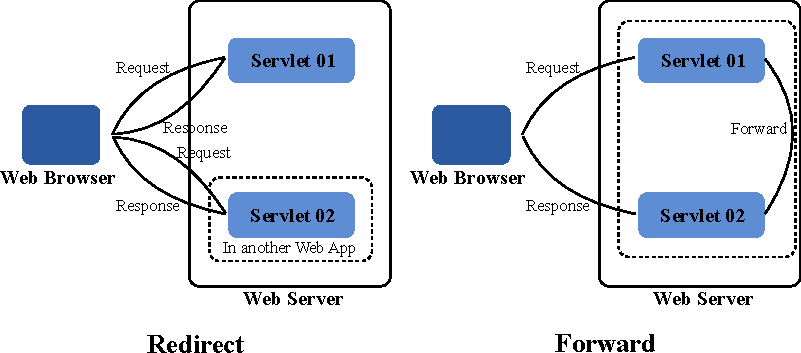
\includegraphics[width=0.9\textwidth]{fig01.pdf}
\end{figure}
\end{frame}

\begin{frame}[fragile] % [fragile]参数使得能够插入代码
\frametitle{转发与重定向的区别} 

\begin{enumerate}
\item 发生的地点不同

{\kai 重定向由客户端完成,而转发由服务器完成。}

\item 请求/响应的次数不同

{\kai 重定向两次请求,创建两个请求对象和响应对象,而转发是一次请求,只创建一个请求对象和响应对象。重定向无法共享请求/响应对象,而转发可以。}

\item 目标位置不同

{\kai 重定向可以跳转到Web应用以外的文档,而转发只能在一个Web内部文件中间进行。}
\end{enumerate}
\end{frame}

\begin{frame}[fragile] % [fragile]参数使得能够插入代码
\frametitle{转发编程的注意事项} 

\begin{enumerate}
\item 转发目录与源目录要在同一个目录。
\item 转发之前不应有响应发送,否则导致异常javax.servlet.IllegalStateException抛出。
\item 更改请求目录最好在重定向中。
\end{enumerate}

\end{frame}
%%%%%%%%%%%%%%%%%%%%%%%%%%
\begin{frame}[fragile] % [fragile]参数使得能够插入代码
\frametitle{} 

\end{frame}
%%%%%%%%%%%%%%%%%%%%%%%%%%
%% \begin{figure}
%% \centering
%% 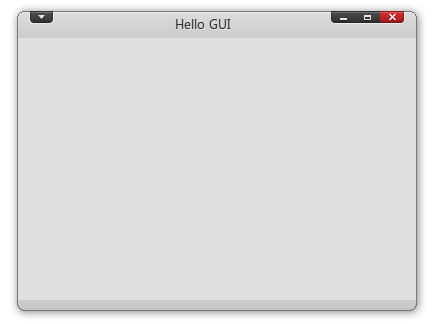
\includegraphics[width=0.6\textwidth]{fig01.png}
%% \end{figure}
% TKS %%%%%%%%%%%%%%%%%%%%%%%%%%%%%%%%%%%%%%%%%%%%%%
\begin{frame}
\centering
{\Huge \textcolor{blue}{THE END}} \\
\vspace{5mm}
{\Large wangxiaodong@ouc.edu.cn} \\
\end{frame}
%%%%%%%%%%%%%%%%%%%%%%%%%%%%%%%%%%%%%%%%%%%%%%%%%%
\end{document}
